\let\negmedspace\undefined
\let\negthickspace\undefined
\documentclass[journal,12pt,onecolumn]{IEEEtran}
\usepackage{cite}
\usepackage{amsmath,amssymb,amsfonts,amsthm}
\usepackage{algorithmic}
\usepackage{graphicx}
\graphicspath{{./figs/}}
\usepackage{textcomp}
\usepackage{xcolor}
\usepackage{txfonts}
\usepackage{listings}
\usepackage{enumitem}
\usepackage{mathtools}
\usepackage{gensymb}
\usepackage{comment}
\usepackage{caption}
\usepackage[breaklinks=true]{hyperref}
\usepackage{tkz-euclide} 
\usepackage{listings}
\usepackage{gvv}                                        
%\def\inputGnumericTable{}                                 
\usepackage[latin1]{inputenc}     
\usepackage{xparse}
\usepackage{color}                                            
\usepackage{array}                                            
\usepackage{longtable}                                       
\usepackage{calc}                                             
\usepackage{multirow}
\usepackage{multicol}
\usepackage{hhline}                                           
\usepackage{ifthen}                                           
\usepackage{lscape}
\usepackage{tabularx}
\usepackage{array}
\usepackage{float}
%\newtheorem{theorem}{Theorem}[section]
%\newthorem{theorem}{Theorem}[section]
%\newtheorem{problem}{Problem}
%\newtheorem{proposition}{Proposition}[section]
%\newtheorem{lemma}{Lemma}[section]
%\newtheorem{corollary}[theorem]{Corollary}
%\newtheorem{example}{Example}[section]
%\newtheorem{definition}[problem]{Definition}

\begin{document}

\title{9.4.33}
\author{EE25BTECH11020 - Darsh Pankaj Gajare}
% \maketitle
% \newpage
% \bigskip
%\begin{document}
{\let\newpage\relax\maketitle}
%\renewcommand{\thefigure}{\theenumi}
%\renewcommand{\thetable}{\theenumi}
Question:\\ Find the roots of the following quadratic equation graphically.
$x^2-4x+3$\\
\solution

The parabola can be expressed in matrix form as
\begin{align}
	\vec{x}^\top \vec{V} \vec{x} + \vec{u}^\top\vec{x} + f = 0
\end{align}
where
\begin{align}
	\vec{V} = \myvec{1 & 0 \\ 0 & 0}, \quad 
    \vec{u} = \myvec{-4 \\ -1}, \quad 
    f = 3.
\end{align}
The line $y=0$ is expressed as:
\begin{align}
    \vec{x} = \vec{q} + \lambda \vec{m}, \quad 
    \vec{q} = \myvec{0 \\ 0}, \quad 
    \vec{m} = \myvec{1 \\ 0}.
\end{align}

Substituting
\begin{align}
	(\vec{q} + \lambda\vec{m})^\top \vec{V} (\vec{q} + \lambda\vec{m}) 
    + \vec{u}^\top(\vec{q} + \lambda\vec{m}) + f = 0.
\end{align}
\begin{align}
	\lambda^2 \brak{\vec{m}^\top \vec{V} \vec{m}}
	+ \lambda \brak{2\vec{q}^\top \vec{V} \vec{m} + \vec{u}^\top \vec{m}}
	+ \brak{\vec{q}^\top \vec{V} \vec{q} + \vec{u}^\top \vec{q} + f} = 0.
\end{align}
\begin{align}
	\vec{m}^\top \vec{V} \vec{m} &= 1, \\
	2\vec{q}^\top \vec{V} \vec{m} + \vec{u}^\top \vec{m} &= -4, \\
	\vec{q}^\top \vec{V} \vec{q} + \vec{u}^\top \vec{q} + f &= 3.
\end{align}

\begin{align}
    \lambda^2 - 4\lambda + 3 = 0.
\end{align}

\begin{align}
    \lambda_1 = 1, \quad \lambda_2 = 3.
\end{align}

Thus, the intersection points are
\begin{align}
    \vec{x}_1 = \myvec{1 \\ 0}, \quad 
    \vec{x}_2 = \myvec{3 \\ 0}.
\end{align}


Plot using C libraries:
\begin{figure}[H]
	\centering
	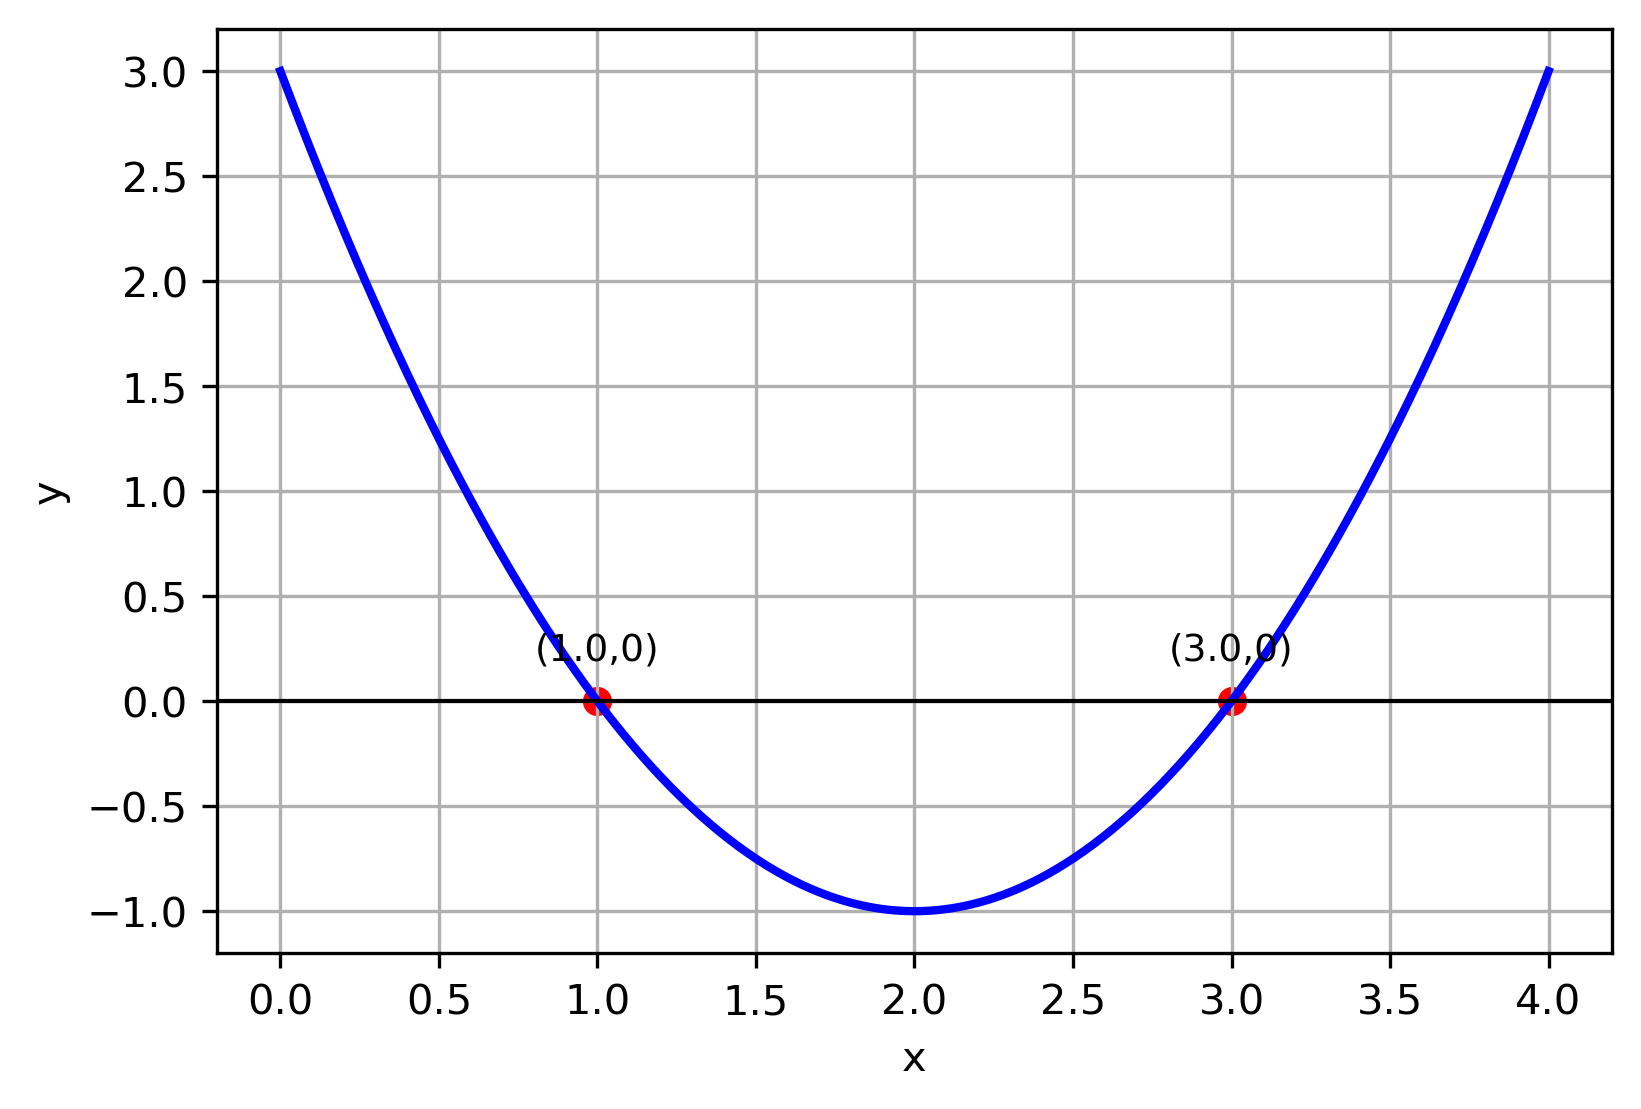
\includegraphics[scale=0.5]{img1}
	\caption*{}
	\label{img1}
\end{figure}
Plot using Python:
\begin{figure}[H]
	\centering
	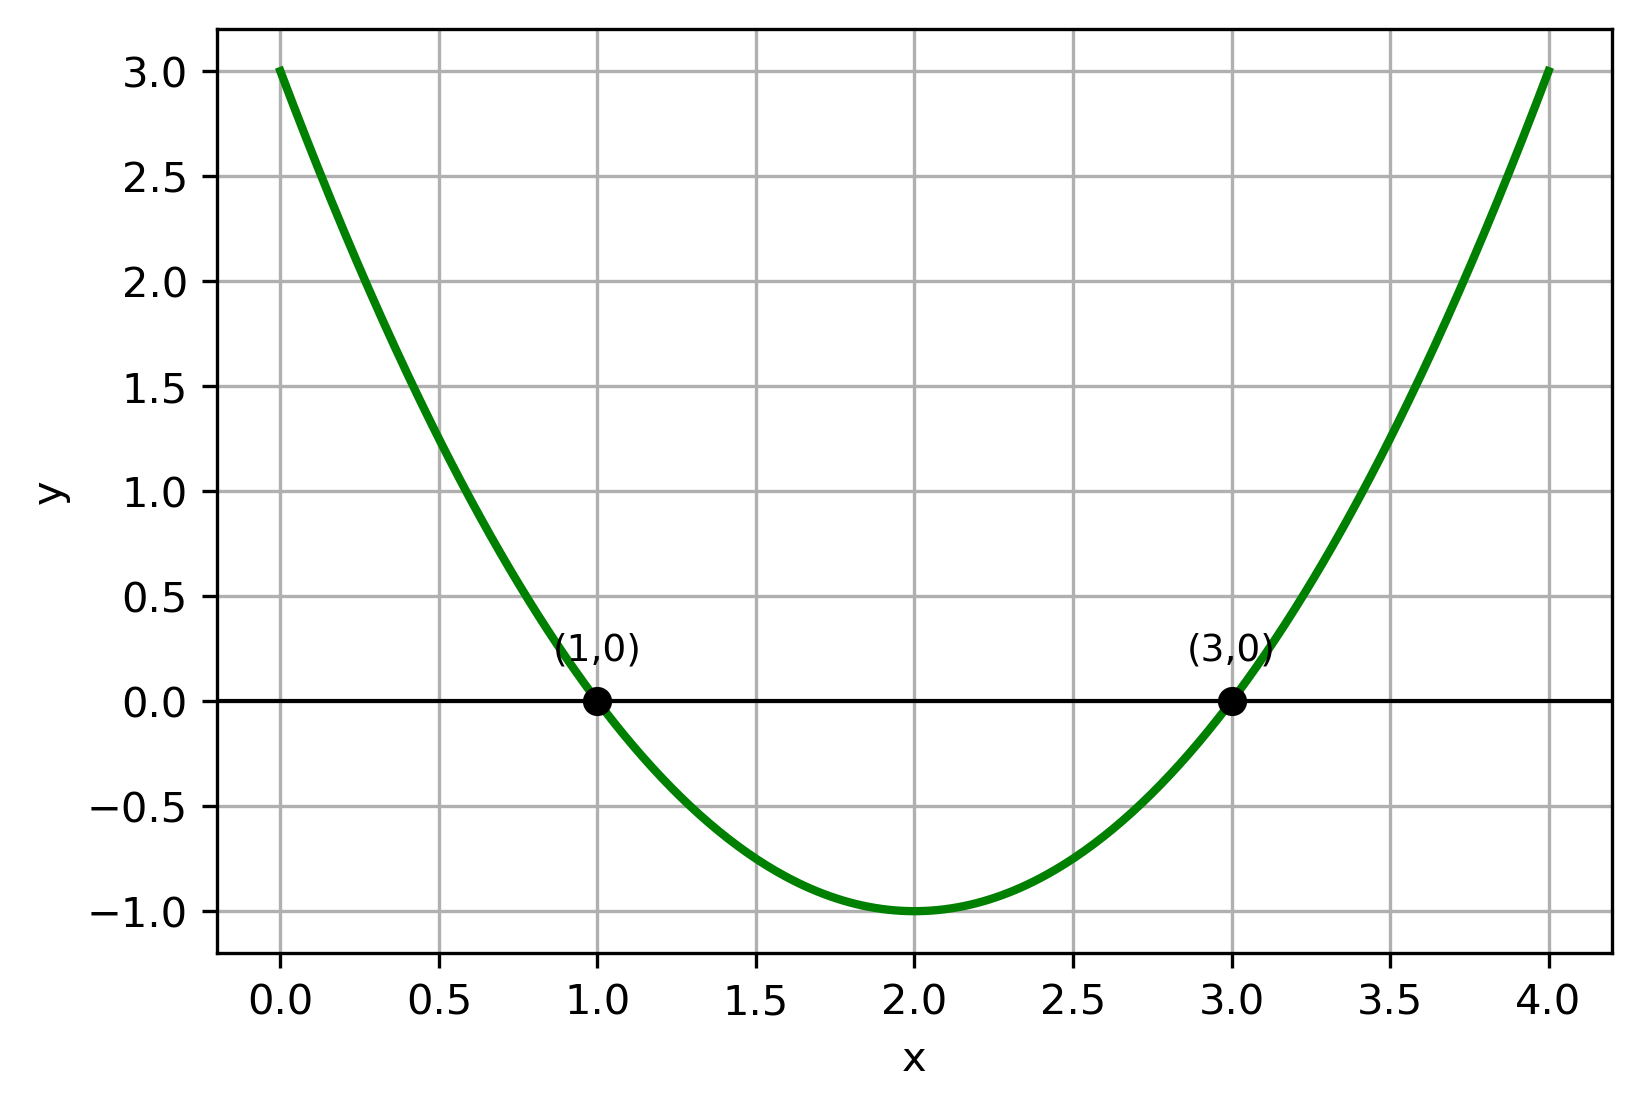
\includegraphics[scale=0.5]{img2}
	\caption*{}
	\label{img2}
\end{figure}
\end{document}

